\section{Exploring the incidents' classification}

\subsection*{Question 4.1}
\textit{Incidents have two types: the type of the incident at the moment it was reported (Initial Type Group) and the type of the incident after it has been studied and classified (Event Clearance Group). Obviously, there should be some kind of correlation of the latter with the former (for instance, incidents reported as robberies are very likely to be also classified finally as robberies). How strong is this correlation?}

The visualization uses a heatmap to show this correlation.
The rows report the incident types at the moment it was reported, while the columns the type it was classified as (we will refer to it as the ``final'' type).
Each cell in the map contains a square, whose area and color are proportional to the number of record for the particular row and column.
Color uses a continuos heat colormap.

The order of rows and columns is initially alphabetical.
However, since there is no $1$-to-$1$ mapping between the categorical values of ``Initial Type Group'' and ``Event Clearance Group'', this order does not have any particular meaning.
Starting from such an order, we have moved some rows and columns to types which seems to be possibly correlated.
For example, ``Initial Type Group'' has the value \textit{Parking Violation}, but ``Event Clearance Group'' does not have it:
we have it closed to \textit{Traffic Related Calls}.

\cref{fig:4_1_initial_vs_final_group_heatmap} shows the visualization.
We can see that:
\begin{itemize}
    \item After some reordering of columns, most of the big squares are along the main diagonal. This means there is a very high correlation between the initial and final types of incidents.
    \item In many cases there is a $1$-to-$1$ match between the initial and final type (e.g. \textit{Disturbances}). In some cases a single initial type matches multiple more specific final types (e.g. \textit{Theft} matches with \textit{Car prowl}, \textit{Other property} and \textit{Shoplifting}).
    \item The first row of the table has a different behaviour. This row represent items without an initial type. They matches different final types, mostly \textit{Disturbances}, \textit{Suspicious circumstances} and \textit{Traffic related calls}.
\end{itemize}

\begin{figure}[h]
	\centering
	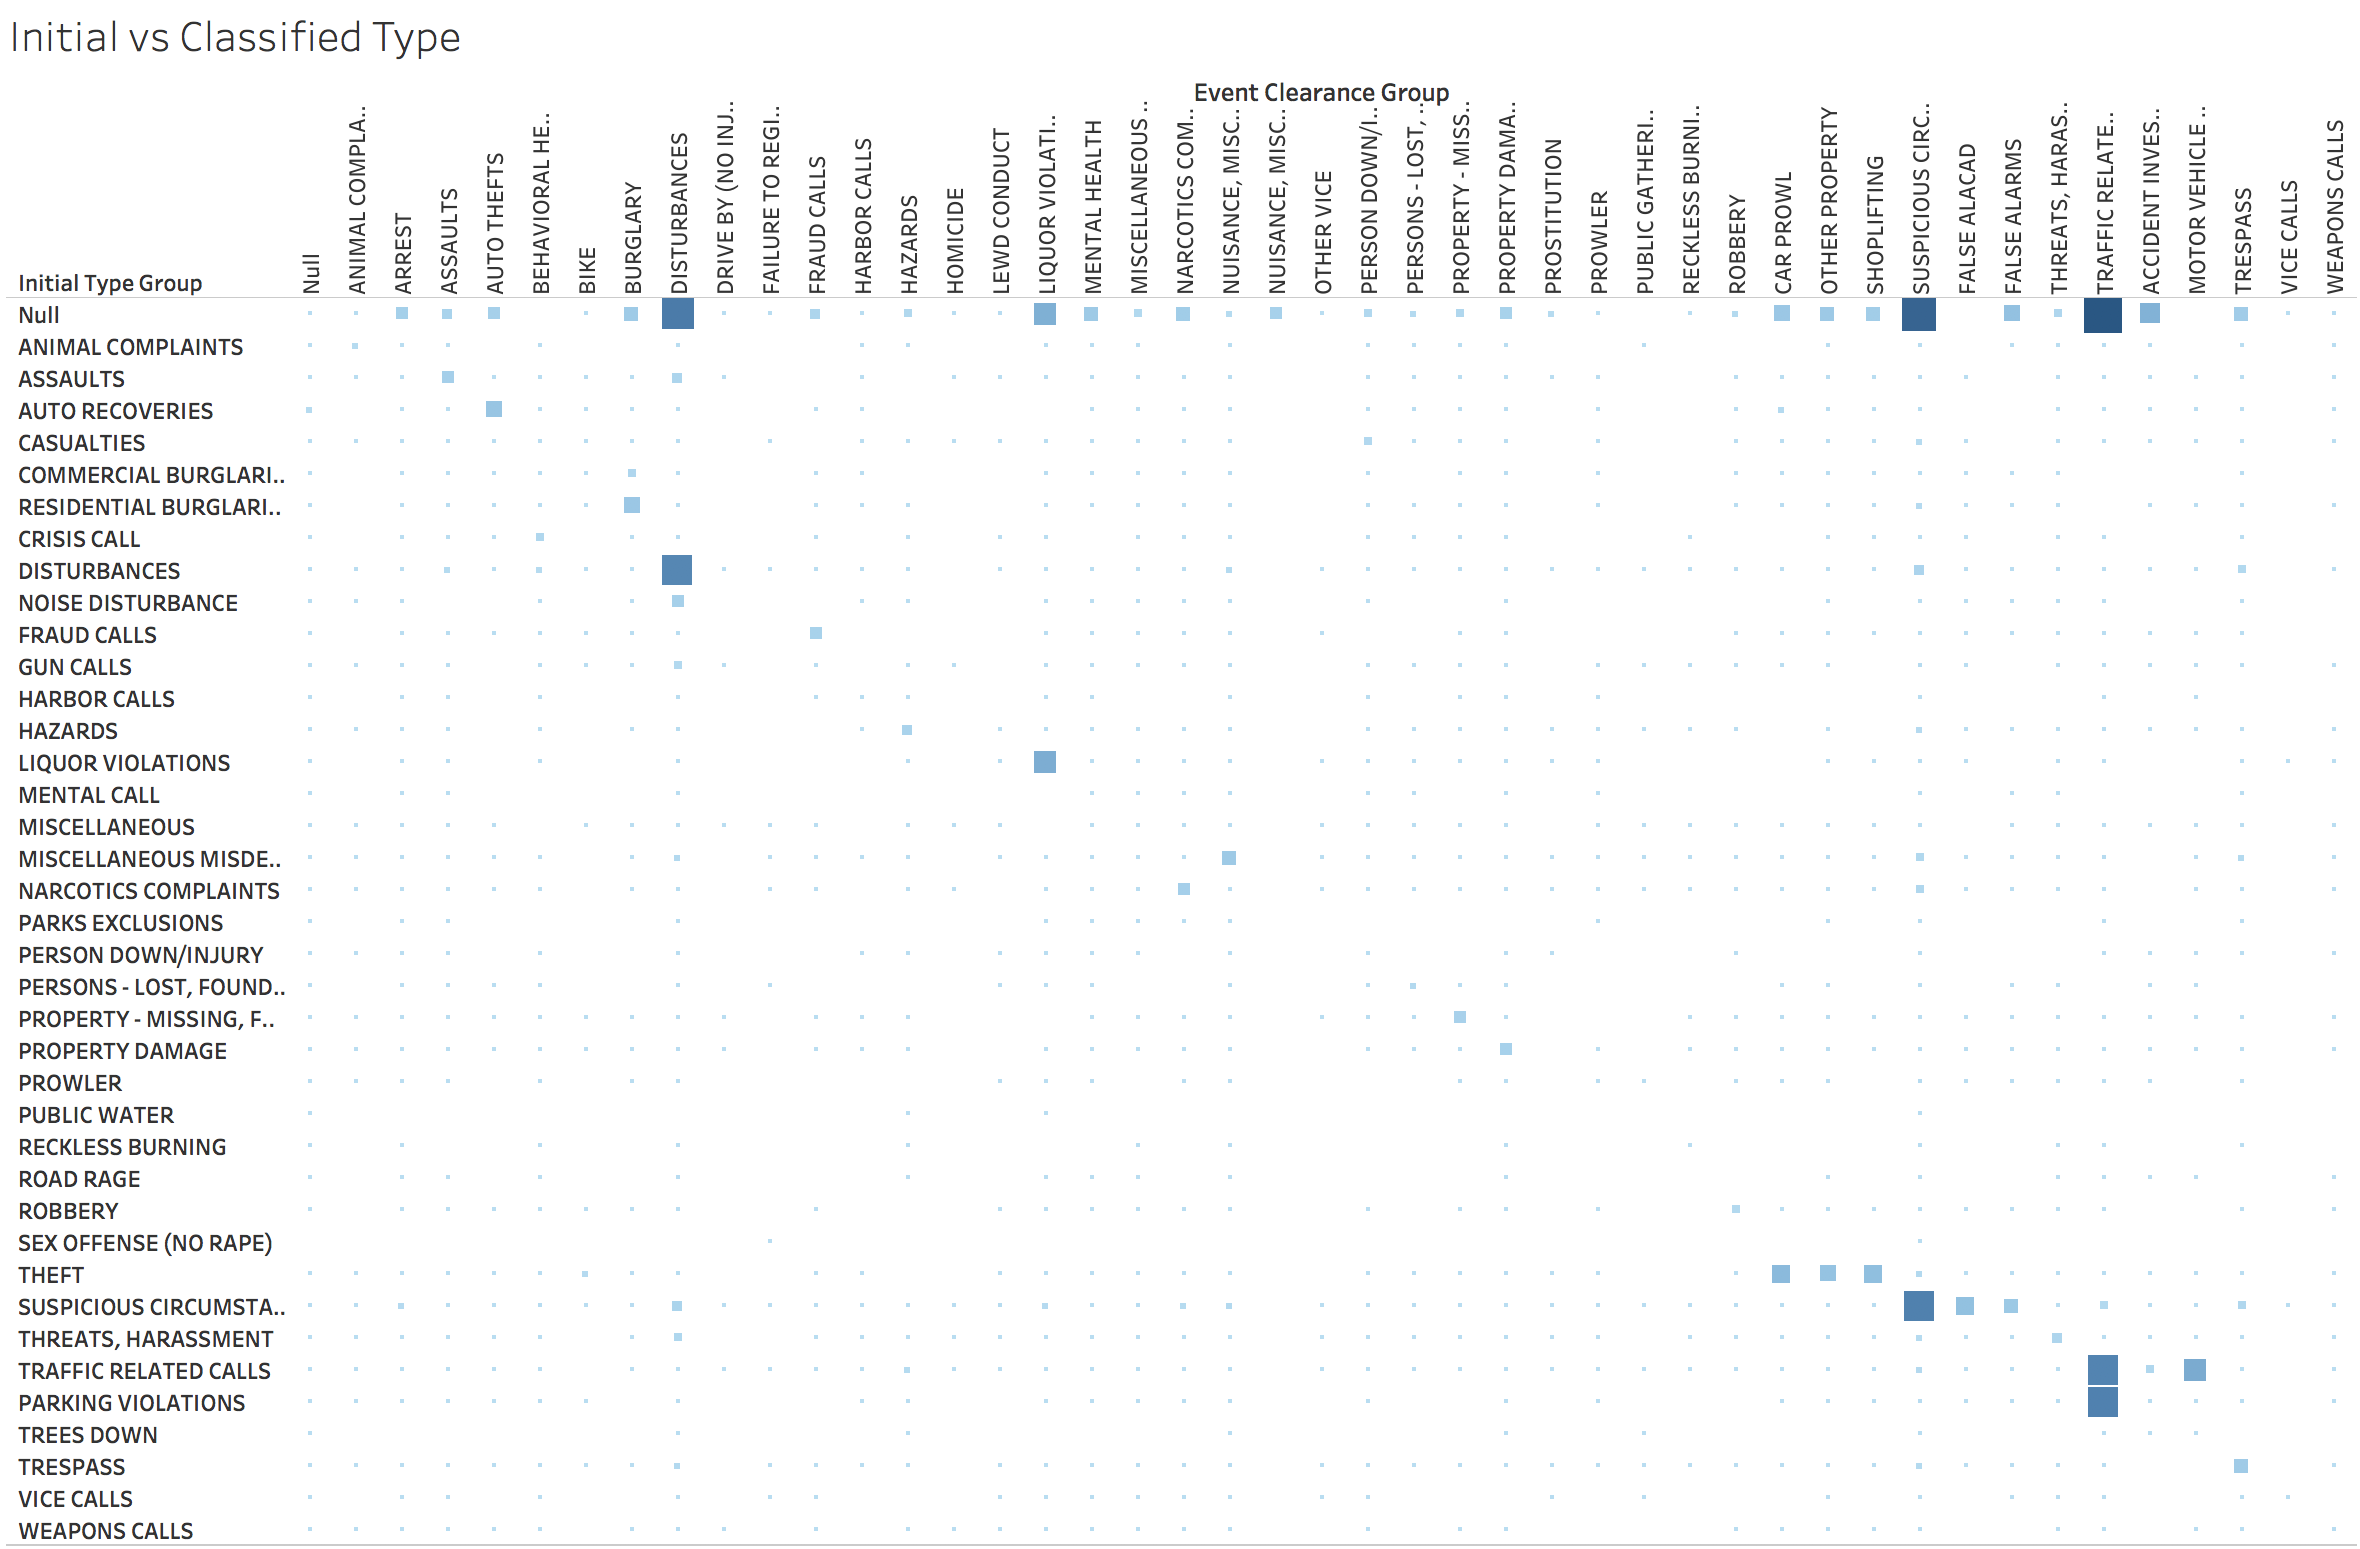
\includegraphics[width=\columnwidth]{figures/4_1_initial_vs_final_group_heatmap}
	\caption{Correlation between the initial and final incident type. The sheet is called ``Initial vs Final Type'' in Tableau.}
	\label{fig:4_1_initial_vs_final_group_heatmap}
\end{figure}

The visualization answers the question, but requires some manual work to find the matching between initial and final types.
Moreover, since most initial types are highly correlated to only a few final ones, it wastes a lot of space.
This makes the square dedicated to interesting correlations very small and difficult to compare with the others.
The use of colors as an overloading helps with that, by does not really solve the problem. 

To better visualize the interesting correlations and remove the manual reordering step, we use a treemap.
We filter out values without an initial type since we have discussed this case previously.
We use the initial type for the first split for the treemap.
Each rectangle corresponds to a pair initial and final types.
Both color and the area of each rectangle encode the number of elements for the particular pair.
Tooltips allows the user to interactively get additional information for each rectangle, namely initial type, final type and number of matching incidents.

\begin{figure}[h]
	\centering
	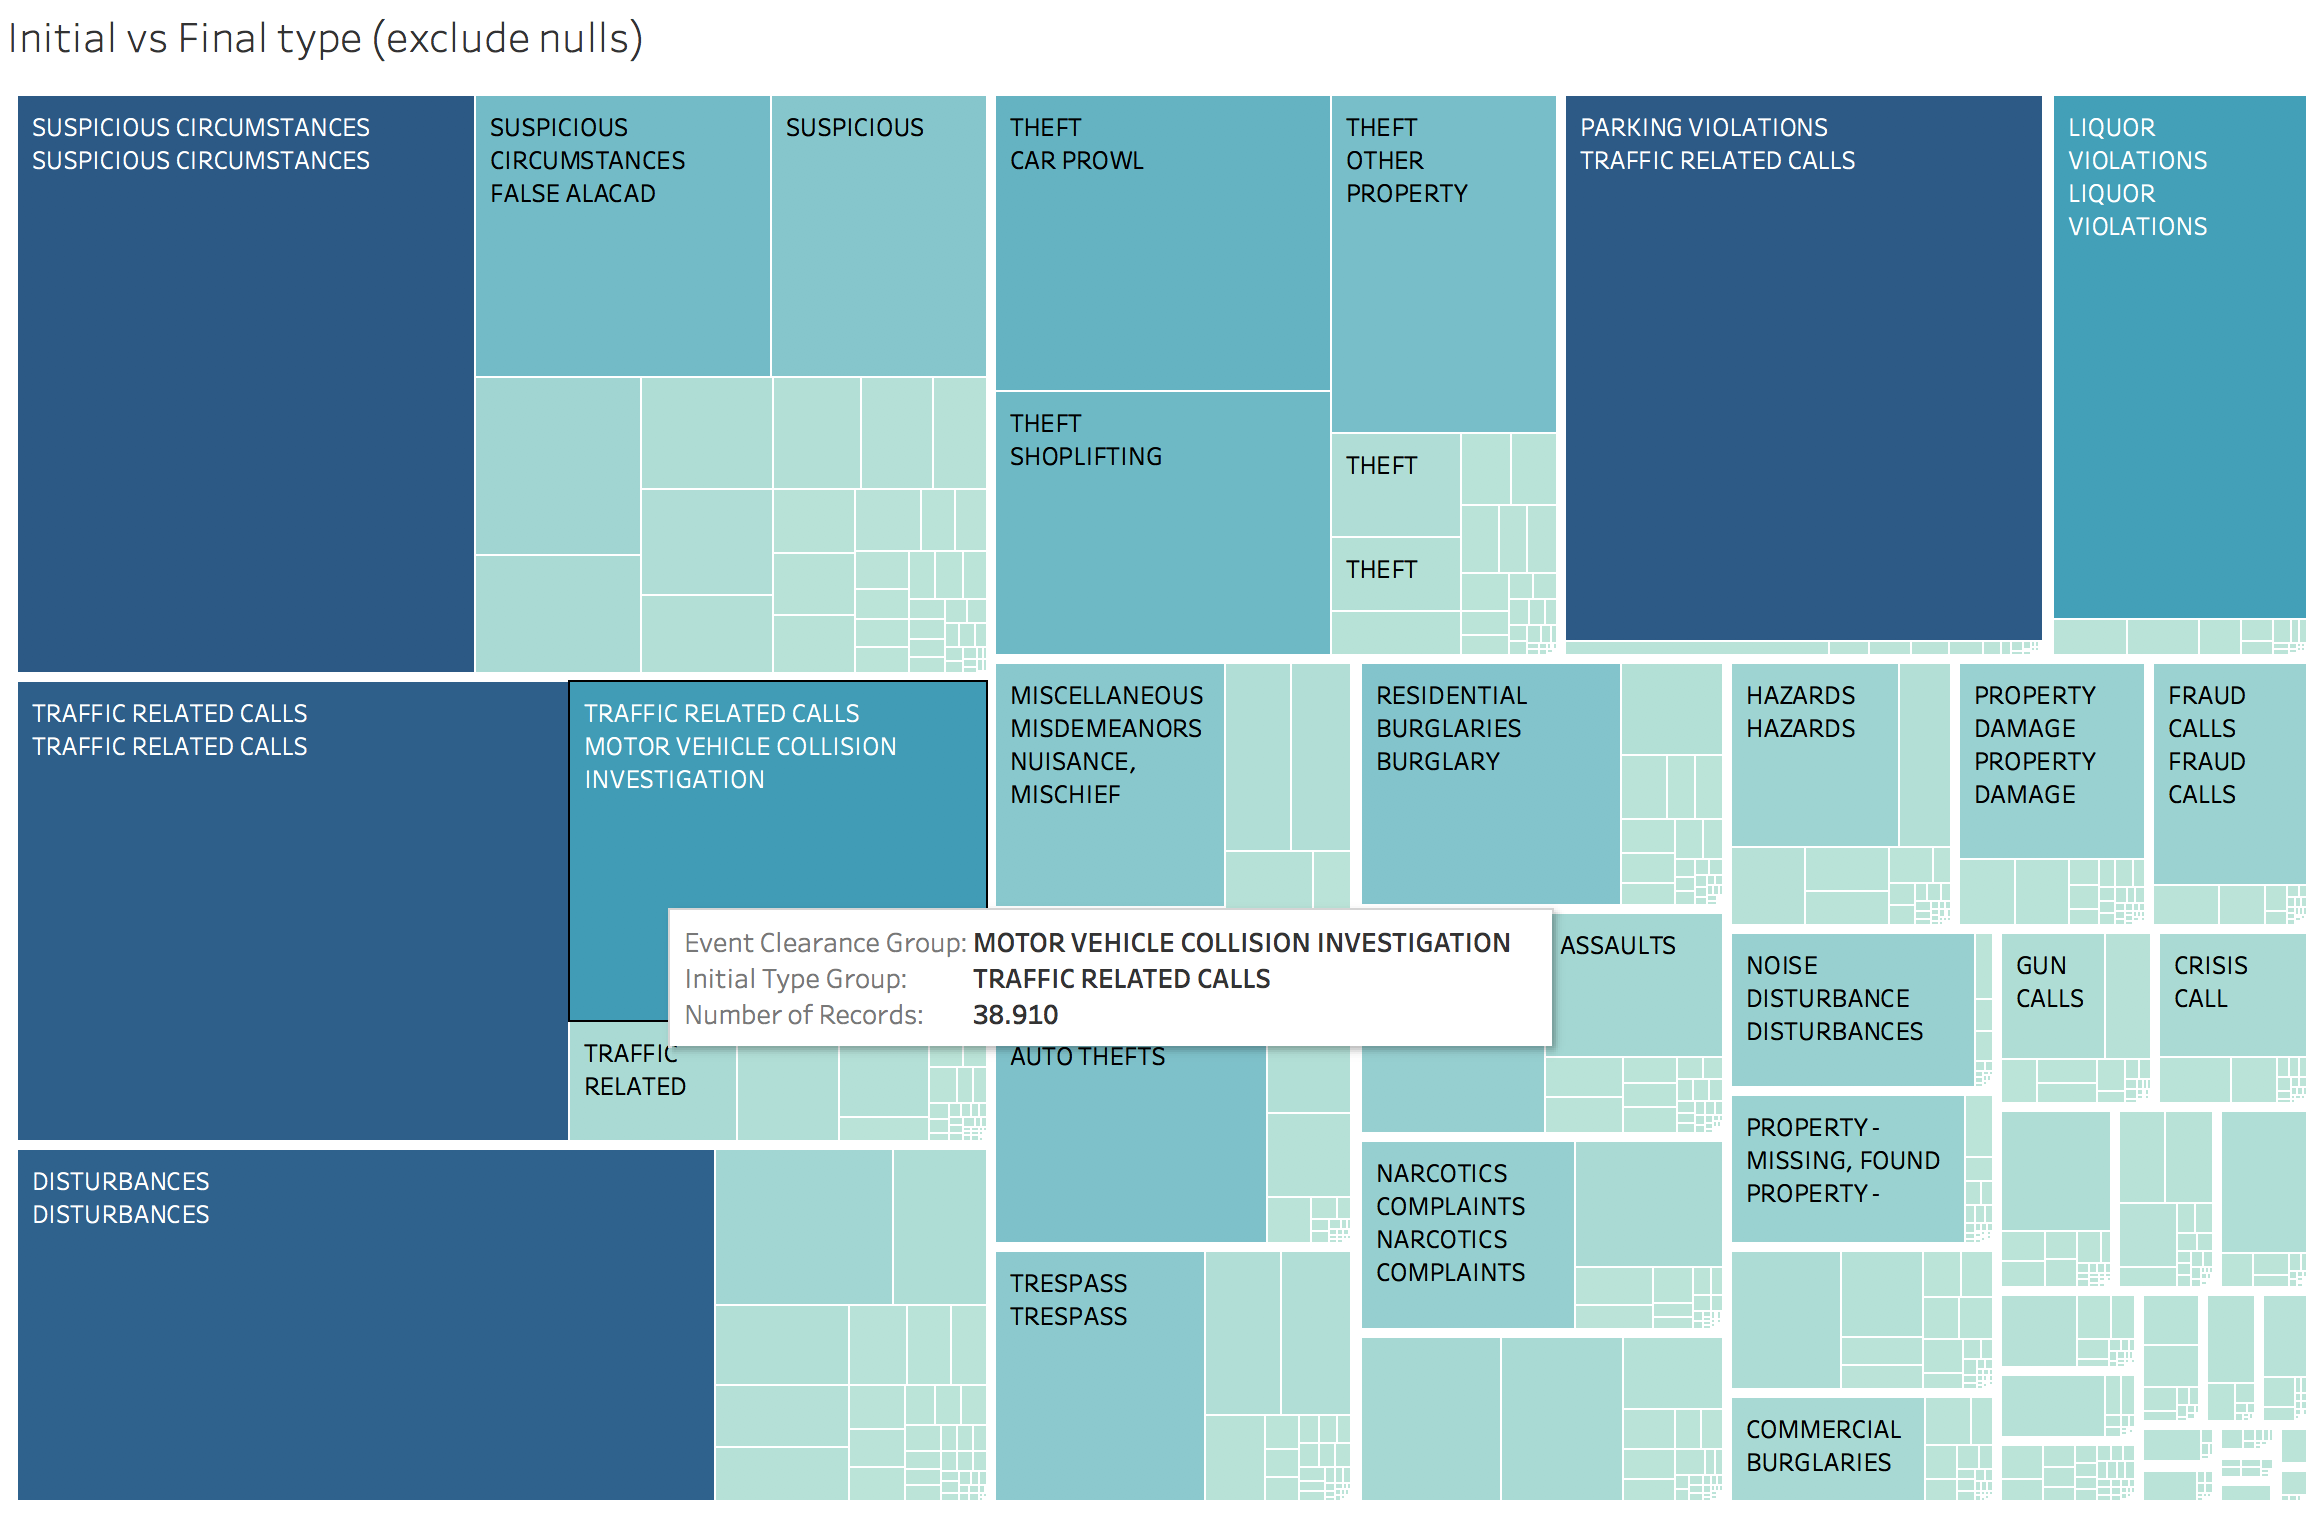
\includegraphics[width=\columnwidth]{figures/4_1_initial_vs_final_group_treemap}
	\caption{Correlation between the initial and final incident type (excluding incidents without an initial type). The sheet is called ``Initial vs Final Type (exclude nulls)'' in Tableau.}
	\label{fig:4_1_initial_vs_final_group_treemap}
\end{figure}

\cref{fig:4_1_initial_vs_final_group_treemap} shows the visualization:
\begin{itemize}
	\item There are some very big rectangles, which indicates a high correlation between the initial and final types.
	\item There are many small rectangles, which indicates a low correlation. For most types the area occupied from small rectangles is negligible, but for some other (e.g. \textit{Suspicious circumstances}) this area is quite relevant. This fact was very difficult to spot in the previous visualization.
	\item Mapping between the initial and final types do not need to be specified interactively by the user. This is the biggest improvement over the previous design.
\end{itemize}

To sum up, there is a quite strong correlation between initial and final types.
However, a lot of incidents with some particular initial cases are often classified in a different way afterwards (e.g. \textit{Suspicious circumstances}).


\subsection*{Question 4.2}
\textit{How do the total number of incidents break down per incident reported type (Initial Type Group) and incident resolution type (Event Clearance Group)?}


\subsection*{Question 4.3}
\textit{How do the total number of incidents break down per incident resolution type (Event Clearance Group) and incident resolution subtype (Event Clearance Subgroup)?}
